\documentclass[]{article}
\usepackage{lmodern}
\usepackage{amssymb,amsmath}
\usepackage{ifxetex,ifluatex}
\usepackage{fixltx2e} % provides \textsubscript
\ifnum 0\ifxetex 1\fi\ifluatex 1\fi=0 % if pdftex
  \usepackage[T1]{fontenc}
  \usepackage[utf8]{inputenc}
\else % if luatex or xelatex
  \ifxetex
    \usepackage{mathspec}
  \else
    \usepackage{fontspec}
  \fi
  \defaultfontfeatures{Ligatures=TeX,Scale=MatchLowercase}
\fi
% use upquote if available, for straight quotes in verbatim environments
\IfFileExists{upquote.sty}{\usepackage{upquote}}{}
% use microtype if available
\IfFileExists{microtype.sty}{%
\usepackage[]{microtype}
\UseMicrotypeSet[protrusion]{basicmath} % disable protrusion for tt fonts
}{}
\PassOptionsToPackage{hyphens}{url} % url is loaded by hyperref
\usepackage[unicode=true]{hyperref}
\hypersetup{
            pdfborder={0 0 0},
            breaklinks=true}
\urlstyle{same}  % don't use monospace font for urls
\usepackage[margin=1in]{geometry}
\usepackage{color}
\usepackage{fancyvrb}
\newcommand{\VerbBar}{|}
\newcommand{\VERB}{\Verb[commandchars=\\\{\}]}
\DefineVerbatimEnvironment{Highlighting}{Verbatim}{commandchars=\\\{\}}
% Add ',fontsize=\small' for more characters per line
\usepackage{framed}
\definecolor{shadecolor}{RGB}{248,248,248}
\newenvironment{Shaded}{\begin{snugshade}}{\end{snugshade}}
\newcommand{\KeywordTok}[1]{\textcolor[rgb]{0.13,0.29,0.53}{\textbf{#1}}}
\newcommand{\DataTypeTok}[1]{\textcolor[rgb]{0.13,0.29,0.53}{#1}}
\newcommand{\DecValTok}[1]{\textcolor[rgb]{0.00,0.00,0.81}{#1}}
\newcommand{\BaseNTok}[1]{\textcolor[rgb]{0.00,0.00,0.81}{#1}}
\newcommand{\FloatTok}[1]{\textcolor[rgb]{0.00,0.00,0.81}{#1}}
\newcommand{\ConstantTok}[1]{\textcolor[rgb]{0.00,0.00,0.00}{#1}}
\newcommand{\CharTok}[1]{\textcolor[rgb]{0.31,0.60,0.02}{#1}}
\newcommand{\SpecialCharTok}[1]{\textcolor[rgb]{0.00,0.00,0.00}{#1}}
\newcommand{\StringTok}[1]{\textcolor[rgb]{0.31,0.60,0.02}{#1}}
\newcommand{\VerbatimStringTok}[1]{\textcolor[rgb]{0.31,0.60,0.02}{#1}}
\newcommand{\SpecialStringTok}[1]{\textcolor[rgb]{0.31,0.60,0.02}{#1}}
\newcommand{\ImportTok}[1]{#1}
\newcommand{\CommentTok}[1]{\textcolor[rgb]{0.56,0.35,0.01}{\textit{#1}}}
\newcommand{\DocumentationTok}[1]{\textcolor[rgb]{0.56,0.35,0.01}{\textbf{\textit{#1}}}}
\newcommand{\AnnotationTok}[1]{\textcolor[rgb]{0.56,0.35,0.01}{\textbf{\textit{#1}}}}
\newcommand{\CommentVarTok}[1]{\textcolor[rgb]{0.56,0.35,0.01}{\textbf{\textit{#1}}}}
\newcommand{\OtherTok}[1]{\textcolor[rgb]{0.56,0.35,0.01}{#1}}
\newcommand{\FunctionTok}[1]{\textcolor[rgb]{0.00,0.00,0.00}{#1}}
\newcommand{\VariableTok}[1]{\textcolor[rgb]{0.00,0.00,0.00}{#1}}
\newcommand{\ControlFlowTok}[1]{\textcolor[rgb]{0.13,0.29,0.53}{\textbf{#1}}}
\newcommand{\OperatorTok}[1]{\textcolor[rgb]{0.81,0.36,0.00}{\textbf{#1}}}
\newcommand{\BuiltInTok}[1]{#1}
\newcommand{\ExtensionTok}[1]{#1}
\newcommand{\PreprocessorTok}[1]{\textcolor[rgb]{0.56,0.35,0.01}{\textit{#1}}}
\newcommand{\AttributeTok}[1]{\textcolor[rgb]{0.77,0.63,0.00}{#1}}
\newcommand{\RegionMarkerTok}[1]{#1}
\newcommand{\InformationTok}[1]{\textcolor[rgb]{0.56,0.35,0.01}{\textbf{\textit{#1}}}}
\newcommand{\WarningTok}[1]{\textcolor[rgb]{0.56,0.35,0.01}{\textbf{\textit{#1}}}}
\newcommand{\AlertTok}[1]{\textcolor[rgb]{0.94,0.16,0.16}{#1}}
\newcommand{\ErrorTok}[1]{\textcolor[rgb]{0.64,0.00,0.00}{\textbf{#1}}}
\newcommand{\NormalTok}[1]{#1}
\usepackage{graphicx,grffile}
\makeatletter
\def\maxwidth{\ifdim\Gin@nat@width>\linewidth\linewidth\else\Gin@nat@width\fi}
\def\maxheight{\ifdim\Gin@nat@height>\textheight\textheight\else\Gin@nat@height\fi}
\makeatother
% Scale images if necessary, so that they will not overflow the page
% margins by default, and it is still possible to overwrite the defaults
% using explicit options in \includegraphics[width, height, ...]{}
\setkeys{Gin}{width=\maxwidth,height=\maxheight,keepaspectratio}
\IfFileExists{parskip.sty}{%
\usepackage{parskip}
}{% else
\setlength{\parindent}{0pt}
\setlength{\parskip}{6pt plus 2pt minus 1pt}
}
\setlength{\emergencystretch}{3em}  % prevent overfull lines
\providecommand{\tightlist}{%
  \setlength{\itemsep}{0pt}\setlength{\parskip}{0pt}}
\setcounter{secnumdepth}{0}
% Redefines (sub)paragraphs to behave more like sections
\ifx\paragraph\undefined\else
\let\oldparagraph\paragraph
\renewcommand{\paragraph}[1]{\oldparagraph{#1}\mbox{}}
\fi
\ifx\subparagraph\undefined\else
\let\oldsubparagraph\subparagraph
\renewcommand{\subparagraph}[1]{\oldsubparagraph{#1}\mbox{}}
\fi

% set default figure placement to htbp
\makeatletter
\def\fps@figure{htbp}
\makeatother


\author{}
\date{\vspace{-2.5em}}

\begin{document}

\section{Using Clojure snippets in
knitr}\label{using-clojure-snippets-in-knitr}

This html document is rendered by R \texttt{knitr} package with embedded
Clojure code. Yes, it's possible. It's even possible by default but the
default version is not usable. The default version is using
\texttt{lein\ exec} and is very, very slow. And doesn't keep session.

This version is configured to use \texttt{nRepl} client,
\href{https://github.com/eraserhd/rep}{\texttt{rep}} which works pretty
well. Add to this Emacs and you get REPL in the Markdown file.

\subsection{What is knitr in short}\label{what-is-knitr-in-short}

Knitr is R package which generates really nice documents out of markdown
file with embed code.

\subsection{First run}\label{first-run}

First let's define \texttt{data}.

\begin{Shaded}
\begin{Highlighting}[]
\NormalTok{(}\BuiltInTok{def}\FunctionTok{ data }\NormalTok{\{}\AttributeTok{:a}\NormalTok{ [}\DecValTok{1} \DecValTok{2} \DecValTok{3}\NormalTok{]}
           \AttributeTok{:b}\NormalTok{ [}\DecValTok{3} \DecValTok{4} \DecValTok{5}\NormalTok{]\})}
\end{Highlighting}
\end{Shaded}

\begin{verbatim}
#'user/data
\end{verbatim}

Code was executed, \texttt{data} is defined and we can run another
chunk.

\begin{Shaded}
\begin{Highlighting}[]
\NormalTok{(}\KeywordTok{keys}\NormalTok{ data)}
\end{Highlighting}
\end{Shaded}

\begin{verbatim}
(:a :b)
\end{verbatim}

And another one.

\begin{Shaded}
\begin{Highlighting}[]
\NormalTok{(}\KeywordTok{->>}\NormalTok{ data}
     \KeywordTok{vals}
\NormalTok{     (}\KeywordTok{apply} \KeywordTok{concat}\NormalTok{)}
\NormalTok{     (}\KeywordTok{reduce} \KeywordTok{+}\NormalTok{))}
\end{Highlighting}
\end{Shaded}

\begin{verbatim}
18
\end{verbatim}

\subsection{Generate image}\label{generate-image}

\begin{Shaded}
\begin{Highlighting}[]
\NormalTok{(}\KeywordTok{require}\NormalTok{ '[clojure2d.core }\AttributeTok{:refer}\NormalTok{ [save]]}
\NormalTok{         '[clojure2d.color }\AttributeTok{:as}\NormalTok{ c]}
\NormalTok{         '[clojure2d.extra.utils }\AttributeTok{:as}\NormalTok{ u])}
\end{Highlighting}
\end{Shaded}

\begin{verbatim}
nil
\end{verbatim}

\begin{Shaded}
\begin{Highlighting}[]
\NormalTok{(}\BuiltInTok{def}\FunctionTok{ img }\NormalTok{(}\KeywordTok{->} \AttributeTok{:cubehelix}
\NormalTok{             (c/gradient)}
\NormalTok{             (u/gradient->image }\VariableTok{true}\NormalTok{)}
\NormalTok{             (save }\StringTok{"docs/gradient.png"}\NormalTok{)))}
\end{Highlighting}
\end{Shaded}

\begin{verbatim}
saving: docs/gradient.png...
...done!
#'user/img
\end{verbatim}

\begin{figure}
\centering

\includegraphics{gradient.png}
\caption{Generated gradient with luma}
\end{figure}

\subsection{How to setup}\label{how-to-setup}

I'm using Emacs with CIDER here.

\begin{itemize}
\tightlist
\item
  Clojure
\item
  Download and install
  \href{https://github.com/eraserhd/rep}{\texttt{rep}}

  \begin{itemize}
  \tightlist
  \item
    Be able to run \texttt{nRepl}
  \end{itemize}
\item
  R

  \begin{itemize}
  \tightlist
  \item
    Install R with \texttt{knitr} package (and all needed deps, like
    \texttt{pandoc})
  \end{itemize}
\item
  Emacs

  \begin{itemize}
  \tightlist
  \item
    Install \texttt{ESS}, \texttt{poly-R} package which enables REPL
    inside Markdown file.
  \end{itemize}
\end{itemize}

Run \texttt{nRepl}, create \texttt{.Rmd} file and add below chunk at the
beginning of it. As you can see, there is a place to define
\texttt{nrepl\_port}. Find your port and change this value. I haven't
been able to find an easy way to setup it automatically (yet).

\begin{Shaded}
\begin{Highlighting}[]
\NormalTok{```\{r setup, include=FALSE\}}
\NormalTok{nrepl_port <- "53247"}
\NormalTok{library(knitr)}
\NormalTok{knitr_one_string <- knitr:::one_string}
\NormalTok{nrepl_cmd  <- "rep"}
\NormalTok{opts_chunk$set(comment=NA, highlight=TRUE)}
\NormalTok{knit_engines$set(clojure = function(options) \{}
\BaseNTok{    code <- paste("-p", nrepl_port, shQuote(knitr_one_string(options$code)))}
\BaseNTok{    out <- if (options$eval) \{}
\BaseNTok{               if (options$message) message('running: ', nrepl_cmd, ' ', code)}
\BaseNTok{               tryCatch(}
\BaseNTok{                   system2(nrepl_cmd, code, stdout = TRUE, stderr = TRUE, env = options$engine.env),}
\BaseNTok{                   error = function(e) \{}
\BaseNTok{                       if (!options$error) stop(e)}
\BaseNTok{                       paste('Error in running command', nrepl_cmd)}
\BaseNTok{                   \}}
\BaseNTok{               )}
\BaseNTok{           \} else ''}
\BaseNTok{    if (!options$error && !is.null(attr(out, 'status'))) stop(knitr_one_string(out))}
\BaseNTok{    engine_output(options, options$code, out)\})}
\NormalTok{```}
\end{Highlighting}
\end{Shaded}

When it's done you can generate documents (html, pdf, whatever) within
\texttt{ESS} or from external R session.

\begin{Shaded}
\begin{Highlighting}[]
\KeywordTok{render}\NormalTok{(}\StringTok{"docs/intro.Rmd"}\NormalTok{,}\StringTok{"all"}\NormalTok{)}
\end{Highlighting}
\end{Shaded}

\subsection{What's odd}\label{whats-odd}

There are couple of problems:

\begin{itemize}
\tightlist
\item
  manual renderer setup
\item
  manual port setup
\item
  no pretty printing results by default
\end{itemize}

\subsection{RMarkdown reference}\label{rmarkdown-reference}

\url{https://bookdown.org/yihui/rmarkdown/}

\subsection{Emacs view}\label{emacs-view}

\begin{figure}
\centering
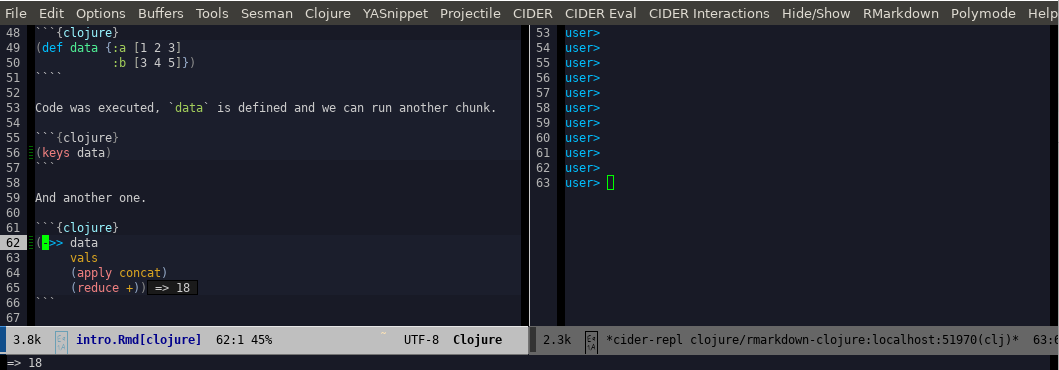
\includegraphics{emacs.png}
\caption{Emacs in action}
\end{figure}

\end{document}
